\documentclass[a4paper,12pt]{article}
\usepackage[indonesian]{babel}
\usepackage{graphicx}
\usepackage{multirow}
\usepackage{enumitem}
\usepackage{listings}
\usepackage{wrapfig}
\usepackage[T1]{fontenc}
\usepackage{inconsolata}
\usepackage{lipsum}
\usepackage{adjustbox}


\usepackage{color}
\usepackage[table]{xcolor}
\definecolor{mygreen}{rgb}{0,0.6,0}
\definecolor{mygray}{rgb}{0.5,0.5,0.5}
\definecolor{mymauve}{rgb}{0.58,0,0.82}
\lstset{%
    language=java,
    showstringspaces=false,          % Prevent tex replacing space to bracket in code
    frame=single,                    % Set frame around code
    backgroundcolor=\color{white},   % choose the background color
    basicstyle=\footnotesize,        % size of fonts used for the code
    breaklines=true,                 % automatic line breaking only at whitespace
    captionpos=b,                    % sets the caption-position to bottom
    commentstyle=\color{mygreen},    % comment style
    keywordstyle=\color{blue},       % keyword style
    stringstyle=\color{mymauve},     % string literal style
}

\graphicspath{ {./img/} }
\begin{document}
\title{ {\Large Laporan Praktikum}\\ Algoritma dan Pemrograman Lanjut\\{\Large Pertemuan 9}}

\author{Aldzikri Dwijayanto Prathama
    \\195410189
    \\Informatika}
\makeatletter
\begin{titlepage}
    \begin{center}
        {\huge \bfseries \@title}\\[14ex]
        
\includegraphics[scale=.8]{logo}\\[4ex]
        {\large \@author}\\[12ex]
        {\large \bfseries {SEKOLAH TINGGI MANAJEMEN INFORMATIKA DAN KOMPUTER
            AKAKOM YOGYAKARTA}}
    \end{center}


%{\large \@date}
\end{titlepage}
\makeatother
%\maketitle
\newpage
\tableofcontents
\newpage

\section{Tujuan}
Mahasiswa dapat menyelesaikan kasus dengan menggunakan method dengan parameter, membuat method overloading dan
menggunakan method-method bawaan yang ada di java

\section{Teori}
\paragraph{}
\begin{enumerate}
    \item Method dengan parameter\\
        Method ada yang mempunyai parameter. Ada 2 buah parameter yaitu
        parameter formal adalah parameter yang tertulis dalam definisi method
        Parameter aktual parameter yang berada pada inputan langsung pada saat
        penggunaan method tersebut.\\

        Parameter bisa lebih dari satu dengan dipisahkan tanda koma. Yang perlu
        diperhatikan pada saat pemanggilan method adalah jumlah, urutan dan tipe
        parameter aktual harus sesuai dengan jumlah urutan dan tipe parameter formal

    \item overloading\\
        Bahasa java mendukung method overloading , java dapat membedakan
        beberapa method dengan nama yang sama di dalam sebuah kelas namun
        parameternya berbeda. Hal ini sangat menguntungkan karena memudahkan kita
        dalam mengingat nama method, bayangkan bila program pada class Gambar
        harus diberi nama drawInterger(int i), drawString(String s), drawDouble(double
        d). Method overloading dibedakan oleh jumlah dan jenis tipe data parameternya
\end{enumerate}

\newpage

\section{Pembahasan}
\subsection{Praktik}
\subsubsection{Praktik 1}
\begin{lstlisting}
public class Fungsi1 {
    public static int jumlah(int a) {
        return a;
    }

    public static void main(String[] args) {
        System.out.println("Hasil pemanggilan methode");
        System.out.println(jumlah(5));
    }
}
\end{lstlisting}

Progran di atas memiliki dua macam parameter, yaitu parameter formal dan parameter aktual. Parameter formal adalah
parameter yang tertulis dalam definisi method.Sedangkan parameter aktual parameter yang berada pada inputan langsung
pada saat penggunaan method tersebut.\\

Method jumlah pada program memiliki pernyataan yang akan mengembalikan nilai dari variabel a, dalam bentuk integer.
Sedangkan method main akan memanggil dan menampilkan hasil dari method jumlah.

\begin{center}
    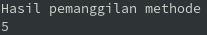
\includegraphics[scale=1]{1.png} 
\end{center}

\subsubsection{Praktik 2}
\begin{lstlisting}
package praktik9;
public class Fungsi2 {
    public static int jumlah(int a) {
        return a;
    }

    public static void main(String[] args) {
        System.out.println("Panggil method jumlah dengan parameter 5");
        System.out.println(jumlah(5));
        System.out.println("Panggil method jumlah dengan parameter 15");
        System.out.println(jumlah(15));
    }
}
\end{lstlisting}
Progran di atas memiliki dua macam parameter, yaitu parameter formal dan parameter aktual. Parameter formal adalah
parameter yang tertulis dalam definisi method.Sedangkan parameter aktual parameter yang berada pada inputan langsung
pada saat penggunaan method tersebut.\\

Method jumlah pada program memiliki pernyataan yang akan mengembalikan nilai dari variabel a, dalam bentuk integer.
Sedangkan method main akan memanggil dan menampilkan hasil dari method jumlah sebanyak 2 kali.

\begin{center}
    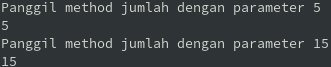
\includegraphics[scale=1]{2.png} 
\end{center}


\subsubsection{Praktik 3}
\begin{lstlisting}
public class Mahasiswa {
    String nim;
    String nama;
    String prodi;

    public void setMhs(String nim, String nama, String prodi) {
        this.nim = nim;
        this.nama = nama;
        this.prodi = prodi;
    }

    public void tampil() {
        System.out.println("NIM: "+ nim);
        System.out.println("Nama: "+ nama);
        System.out.println("Prodi: "+ prodi);
    }

    public static void main(String[] args) {
        Mahasiswa mhs = new Mahasiswa();
        mhs.setMhs("145410012", "Nisa", "Informatika");
        mhs.tampil();
    }
}
\end{lstlisting}
Program pada praktik 3 ini memiliki 3 buah method, dan variabel yang dideklarasikan secara global. Method setMhs
berfungsi untuk menginisialisasi nilai pada variabel nim, nama, dan prodi secara globa. Method tampil berfungsi untuk
menampilkan nim, nama, dan prodi. Sedangkan method main berfungsi untuk memanggil method dengan menciptakan objek, dan
memasukkan nilai ke variabel.

\begin{center}
    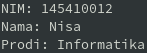
\includegraphics[scale=1]{3.png} 
\end{center}


\subsubsection{Praktik 4}
\begin{lstlisting}
public class DemoOverload {
    void sum(int a, int b) {
        System.out.println(a + b);
    }

    void sum(int a, int b, int c) {
        System.out.println(a + b + c);
    }

    public static void main(String[] args) {
        DemoOverload demo = new DemoOverload();
        demo.sum(1,6);
        demo.sum(4,2,3);
    }
}
\end{lstlisting}
Program di atas memiliki method overloading, yakni method dengan nama yang sama di dalam sebuah kelas namun
parameternya berbeda. Pada program ini, method sum pertama memiliki dua parameter integer, sedangkan method sum kedua
memiliki 3 parameter integer. Kemudian pada method main, dipanggil method sum dengan membuat objek baru, lalu dipanggil
dengan memberikan parameter yang berbeda.

\begin{center}
    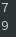
\includegraphics[scale=1]{4.png} 
\end{center}


\subsubsection{Praktik 5}
\begin{lstlisting}
public class StringComparisonExample {
    public static void main(String[] args) {
        String tv = "Bravia";
        String television = "Bravia";

        if (tv.equals(television)) {
            System.out.println("Both tv and television contains same letters and equal byequals method od String");
        }

        if (tv.compareTo(television) == 0) {
            System.out.println("Both tv and television are equal using compareTo method of String");
        }

        television = "BRAVIA";

        if (tv.equalsIgnoreCase(television)) {
            System.out.println("tv and television are equal by equalsIgnoreCase method of String");
        }

        if (tv.compareToIgnoreCase(television) == 0) {
            System.out.println("tv and television are same by compareToIgnoreCase of String");
        }

        String sony = "Sony";
        String samsung = "Samsung";

        if (sony.compareTo(samsung) > 0) {
            System.out.println("Sony comes after Samsung in lexicographical order");
        } else if (sony.compareTo(samsung) < 0) {
            System.out.println("Sony comes before Samsung in lexicographical order");
        }
    }
}
\end{lstlisting}

Program pada praktik 5 menggunakan beberapa method bawaan java. Method pertama yaitu equals, yang membandingkan strings
antara variabel tv dan television, dan akan menghasilkan nilai true jika string pada kedua variabel tersebut sama.\\

Method kedua yaitu compareTo, method ini membandingkan dua string berdasarkan nilai unicode pada setiap karakter di
dalam string.\\

Method ketiga adalah equalsIgnoreCase, method ini membandingkan strings dengan menghiraukan kapitalisasi pada
karakter.\\

Method selanjutnya adalah compareToIgnoreCase, method ini membandingkan nilai unicode karakter, tetapi huruf besar dan
kecil dianggap sama selama alphabetnya sama.

\begin{center}
    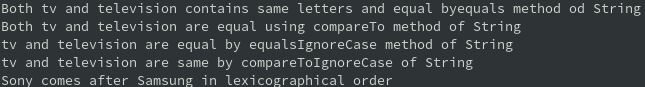
\includegraphics[width=.8\linewidth]{5.png} 
\end{center}

\subsection{Latihan}
Memodifikasi praktik 3 sehingga dapat menampilkan IPK.\@
\begin{lstlisting}
public class Mahasiswa1 {
    String nim;
    String nama;
    String prodi;
    double ipk;

    public void setMhs(String nim, String nama, String prodi, double ipk) {
        this.nim = nim;
        this.nama = nama;
        this.prodi = prodi;
        this.ipk = ipk;
    }

    public void tampil() {
        System.out.println("NIM: "+ nim);
        System.out.println("Nama: "+ nama);
        System.out.println("Prodi: "+ prodi);
        System.out.println("IPK : "+ ipk);
    }

    public static void main(String[] args) {
        Mahasiswa1 mhs = new Mahasiswa1();
        mhs.setMhs("145410012", "Nisa", "Informatika", 3.9);
        mhs.tampil();
    }
}
\end{lstlisting}

Agar program dapat dimasukkan dam mengeluarkan IPK, maka ditambahkan variabel ipk secara global. Kemudian pada method
setsetMhs ditambahkan pernyataan untuk menginisialisasi nilai pada variabel ipk. Pada method tampil ditambahkan
pernyataan untuk menampilkan variabel IPK pada layar. Untuk method main ditambahkan nilai IPK yang akan dimasukkan.

\begin{center}
    
\includegraphics[scale=1]{6.png} 
\end{center}


\subsection{Tugas}
\begin{lstlisting}
import java.util.Scanner;
public class Tugas {

    public static void main(String[] args) {

        Scanner in = new Scanner(System.in);
        double bil = in.nextInt();
        in.close();
        System.out.printf("Akar kuadrat dari %.3f adalah %.3f %n", bil, Math.sqrt(bil));
    }
}
\end{lstlisting}
Program Tugas tersebut menggunakan method bawaan java sqrt, yaitu method yang berfungsi untuk menghitung akar dua dari
sebuah bilangan.

\begin{center}
    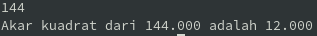
\includegraphics[scale=1]{7.png} 
\end{center}


\newpage

\section{Kesimpulan}
Setelah praktik mahasiswa dapat menyelesaikan kasus dengan menggunakan method dengan parameter, membuat method overloading dan
menggunakan method-method bawaan yang ada di java

\end{document}
